
\item A solid body rotates about a stationary axis according to the law $\varphi = at - bt^3$, where $a = 6.0 \text{ rad/s}^2$ and $b = 2.0 \text{ rad/s}^3$. Find:
    \begin{center}
        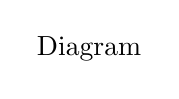
\begin{tikzpicture}
            \node at (0, 0) {Diagram}; % Replace this with the actual diagram code
        \end{tikzpicture}
    \end{center}
    \begin{enumerate}
        \item the mean values of the angular velocity and angular acceleration averaged over the time interval between $t = 0$ and the complete stop;
        \item the angular acceleration at the moment when the body stops.
    \end{enumerate}
